\chapter{Life chaos} \label{cap:caos-della-vita}

Now we want to give the Turtle the ability to take decisions but first let's make the scenario more interesting. 

So far we have depicted a sort of deterministic vision of computer programming. In our context this means giving the Turtle clear commands - do this, do that. Once the program is written the game is over. No matter the complexity, the drawing is frozen in the code. Thus, there is no place for randomness in the computer? Yes and no. A technical explanation for this answer would be too complex here. In a first approximation we can say that, no, a computer cannot produce true randomness but a sort of pseudo-randomness, thanks to appropriate mathematical tricks\footnote{Basically, in order to produce randomness one has to be able to generate random numbers, by means of so called random number generators. In reality, they generate periodic sequences, in the sense that after a certain number of numbers the same initial sequence is started again. The trick consists in using algorithms that produce extremely large periods so that one never reaches the end of the sequence by means of successive number extractions.}.

The Turtle understands the RANDOM command:

\begin{itemize}
\item X = RANDOM 100 ; gives back a random float\footnote{In computer science a float number is a number with decimal digits. For instance, 3.14 is a float number, 18 is an integer number.} number (0 <= X < 100), that is equal or greater than 0 and smaller than 100
\item X = RANDOM “abcde” ; gives back a random letter among a, b, c, d, e
\item X = RANDOM [1, 2, 3] ; gives back a random element among 1, 2 and 3 - you can also mix different items, for instance RANDOM [1, “pippo”, 3.14]
\end{itemize}

In the aforementioned examples the random choices are memorized in the variable named X. Of course you can choose whatever name you prefer, or even use the instructions in some different way. For instance, try to play with the different use of the RANDOM command by means of the following code:

\vskip 1cm

\begin{scriptsize}
\begin{minipage}{0.50\textwidth}
\begin{itemize}[itemsep=-3pt,parsep=2pt, leftmargin=-0.0mm ]
\item[] HOME
\item[] CLEARSCREEN 
\item[] 
\item[] PENUP
\item[] FORWARD 300
\item[] 
\item[] REPEAT 10 [
\item[] \hspace{8pt} LABEL RANDOM 100
\item[] \hspace{8pt} BACK 12
\item[] ]                      
\end{itemize}
\end{minipage}
\end{scriptsize}
\begin{minipage}{0.5\textwidth}
\begin{figure}[H]
   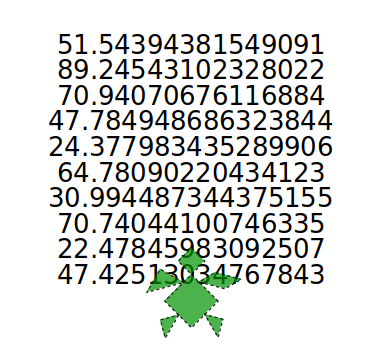
\includegraphics[width=3.0cm,trim=4 4 8 4,clip]{./images/caos-della-vita/caos-della-vita-1.png}
   \label{dec-2}
\end{figure}
\end{minipage} \hfill

\vskip 1cm

With this code the Turtle first goes next to the page top, then writes a column of ten successive random numbers between 0 and 100, printing them by means of the LABEL instruction. Of course you can change whatever you like in this piece of code - it's always good to experiment.

Now, let's take a basic piece of code we are using several times, with variants:

\vskip 1cm

\begin{scriptsize}
\begin{minipage}{0.50\textwidth}
\begin{itemize}[itemsep=-3pt,parsep=2pt, leftmargin=-0.0mm ]
\item[] TO QUADRATO                 
\item[] \hspace{8pt} 	REPEAT 4 [ 
\item[] \hspace{8pt}\hspace{8pt}		FORWARD 100 
\item[] \hspace{8pt}\hspace{8pt}		RIGHT 90
\item[] \hspace{8pt}	]
\item[] END                            
\item[] 
\item[] QUADRATO
\end{itemize}
\end{minipage}
\end{scriptsize}

\vskip 1cm

This is the code to draw a square, as we have seen at the beginning of chapter \ref{cap:disegnare}. In chapter \ref{cap:ripetere} we investigated how to transform this code to get any kind of regular polygons. In a somewhat more complex variant, in chapter \ref{cap:marta}) we will explore more general cycles properties and in chapter \ref{cap:cerchio} we will discover the natural way of drawing a circle in the Turtle Geometry perspective, put in a practical didactic perspective: here just the code, to point out the similarity with the previous one.

\vskip 1cm

\begin{scriptsize}
\begin{minipage}{0.50\textwidth}
\begin{itemize}[itemsep=-3pt,parsep=2pt, leftmargin=-0.0mm ]
\item[] TO CERCHIO                 
\item[] \hspace{8pt} 	REPEAT 360 [ 
\item[] \hspace{8pt}\hspace{8pt}		FORWARD 1 
\item[] \hspace{8pt}\hspace{8pt}		RIGHT 1
\item[] \hspace{8pt}	]
\item[] END                            
\item[] 
\item[] CERCHIO
\end{itemize}
\end{minipage}
\end{scriptsize}

\vskip 1cm

Now, we have all the ingredients to give life to our Turtle. Let's inject a dose of randomness in the previous code. Within the repeating cycle, first we are going to tell the Turtle to move forward by a random amount between 1 and 2. In order to achieve this effect we write the instruction FORWARD RANDOM(1) + 1.  Here we are telling the Turtle to move forward by a quantity equal to RANDOM(1) +1. The command RANDOM(1)\footnote{At the beginning we showed a slightly different syntax: RANDOM 1 instead RANDOM(1). The first one is the standard LibreLogo version reported in the official LibreLogo Toolbar manual. The second one is an alternative version which is based on the underlying python code by means of which LibreLogo has been written. In the example we are discussing this version is preferable because it gives more clarity. Actually,  with the expression RANDOM 1 + 1 it is not clear if we are willing to sum 1  to the result of RANDOM 1 or if we want to call RANDOM 2. By using RANDOM(1) + 1 there is not such an ambiguity. } renders a random number between 0 and 1, thus, if we sum 1 to this, we obtain a random number which is comprised between 1 and 2. Second, we tell the Turtle to turn by a random amount, say between -45 and 45 degrees. We can achieve this result simlarly, by means of the instruction LEFT RANDOM(90) - 45, since with RANDOM(90) - 45 we get a random number between -45 and 45 degrees. 

Here we have the whole piece of code and its result:

\vskip 1cm

\begin{scriptsize}
\begin{minipage}{0.50\textwidth}
\begin{itemize}[itemsep=-3pt,parsep=2pt, leftmargin=-0.0mm ]
\item[] TO RANDOMMOVE
\item[] \hspace{8pt} 	REPEAT [ 
\item[] \hspace{8pt}\hspace{8pt}		FORWARD RANDOM(1) + 1 
\item[] \hspace{8pt}\hspace{8pt}		RIGHT RANDOM(90) - 45
\item[] \hspace{8pt}	]
\item[] END                            
\item[] 
\item[] RANDOMMOVE
\end{itemize}
\end{minipage}
\end{scriptsize}
\begin{minipage}{0.5\textwidth}
\begin{figure}[H]
   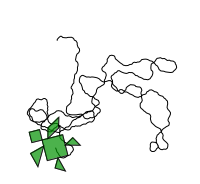
\includegraphics[width=3.0cm,trim=4 4 8 4,clip]{./images/caos-della-vita/caos-della-vita-2.png}
   \label{dec-2}
\end{figure}
\end{minipage} \hfill

\vskip 1cm

If these code modifications sound weird to you, just play with it. That is copy the code in a new LibreOffice document, try to run it, then try to modify the various numbers and reflect upon what's happening. 

But be aware: if you are going to run repeatedly the same piece of code you will not be able to reproduce this drawing, or better: the probability of reproducing the same drawing is extremely low. So what? How can we be happy of producing unpredictable results by means of a machine conceived for making complex and accurate calculations? Well, actually, we are very glad because with this simple code we open a windows on the huge and crucial world of scientific simulation. Nowadays, in every scientific field the simulation is an essential investigation tool, the unique possible to face the overwhelming complexity of natural phenomena. However, nowadays does not mean right today. My graduation thesis in physics, in the seventies, was heavily based on the use of computer simulation of radiation scattering within the human body. A too complex context to be faced with the tools of mathematical analysis. In physics computer simulations make use of so called Monte Carlo Methods, a broad class of computational algorithms that rely on repeated random sampling to obtain numerical results. For instance, in my thesis work, I simulated a source of radioactivity within the body, by reproducing the emission of photons, thus invoking a random number generator for any random step, such as direction of emission, interaction with matter, direction of deflection and so on. 

But simulations are not restricted to the domain of physics, on the contrary, the more complex the phenomena the more simulations may turn out to be the unique possible investigation tool. In the context of biological disciplines we talk about \textit{in silico} experiments, referring to the fact that they are realized through calculations done with digital computers that run on silicon chips - the expression is an allusion to the latin phrases \textit{in vivo}, \textit{in vitro} and \textit{in situ}, commonly used in biology. Nowadays \textit{in silico} experiments include molecular biology, genetic assays, tumour growth, dermatology, bone remodelling, organ failure, clinical trials, just to mention some. In medicine, for instance, \textit{in silico} studies are used to discover new drugs because it is faster and costs much less. In biology they are used to study to formulate behaviour model of cells and in genetics to analyze gene expression\footnote{In molecular biology "gene expression" means the way a set of genes determines  the functioning of the cell at the macromolecular level}. 

But what are we simulating with our piece of code? The obvious answer is a turtle wandering randomly. Of course, if we imagine to observe an animal from the height in its environment,  the impression will be that of a random movement.  In this sense our code could be considered a simulation of the animal behaviour, even if a very poor one, since our randomness assumption is based on the fact that we ignore what the animal is actually doing. Animals move because they are looking for food or a mate, for instance. Or, perhaps, the simulation could be more appropriate for a drunk hanging around in the night, looking for a nonexistent happiness. The distribution of food for a given specie of animals in its natural environment could be modeled, in some extent, but the inner struggle of a man is much more difficult to translate in mathematical terms. 

But what does it mean exactly by "modeling something", such as food distribution, in the context of our example? Yes, apparently, we injected a drop of life in our code, reproducing a randomness which we all experience in our life, in the shape of good or bad luck. However, despite such strong perception of uncertainty, we all know that our capability of observing the outside world and of tacking decisions, is crucial, as well. In substance, our turtle is totally passive! It just have some energy to proceed and to turn: no smell, no sight, no decisions. This is the point: we need a way to let the Turtle have the ability to take decisions!

Before going on learning how to let the Turtle take decisions, we diverge a bit from the LibreLogo environment to have a fast look to the fascinating world of \textit{multiple turtles}. We have to give up to LibreLogo for a while because it does not allow to run more turtles simultaneously, at least in the current version. It is plenty of Logo versions out there, and some of them allow to run more then one turtle at a time. As we have already said, the reason for using LibreLogo as the first but not trivial introduction to Logo relies in its extremely \textit{low floor}, which is crucial in primary school. 

\vskip 1cm\chapter{Taking decisions} \label{cap:decisioni}

Now we want to give the Turtle the ability to take decisions but first let's make the scenario more interesting.

So far we have depicted a sort of deterministic vision of computer programming. In our context this means giving the Turtle clear commands - do this, do that. Once the program is written the game is over. No matter the complexity, the drawing is frozen in the code. Thus, there is no place for randomness in the computer? Yes and no. A technical explanation for this answer would be too complex here. In a first approximation we can say that, no, a computer cannot produce true randomness but a sort of pseudo-randomness, thanks to appropriate mathematical tricks\footnote{Basically, in order to produce randomness one has to be able to generate random numbers, by means of so called random number generators. In reality, they generate periodic sequences, in the sense that after a certain number of numbers the same initial sequence is started again. The trick consists in using algorithms that produce extremely large periods so that one never reaches the end of the sequence by means of successive number extractions.}.

The Turtle understands the RANDOM command:

\begin{itemize}
\item X = RANDOM 100 ; gives back a random float\footnote{In computer science a float number is a number with decimal digits. For instance, 3.14 is a float number, 18 is an integer number.} number (0 <= X < 100), that is equal or greater than 0 and smaller than 100
\item X = RANDOM “abcde” ; gives back a random letter among a, b, c, d, e
\item X = RANDOM [1, 2, 3] ; gives back a random element among 1, 2 and 3 - you can also mix different items, for instance RANDOM [1, “pippo”, 3.14]
\end{itemize}

In the aforementioned examples the random choices are memorized in the variable named X. Of course you can choose whatever name you prefer, or even use the instructions in some different way. For instance, try to play with the different use of the RANDOM command by means of the following code:

\vskip 1cm

\begin{scriptsize}
\begin{minipage}{0.50\textwidth}
\begin{itemize}[itemsep=-3pt,parsep=2pt, leftmargin=-0.0mm ]
\item[] HOME
\item[] CLEARSCREEN
\item[]
\item[] PENUP
\item[] FORWARD 300
\item[]
\item[] REPEAT 10 [
\item[] \hspace{8pt} LABEL RANDOM 100
\item[] \hspace{8pt} BACK 12
\item[] ]
\end{itemize}
\end{minipage}
\end{scriptsize}
\begin{minipage}{0.5\textwidth}
\begin{figure}[H]
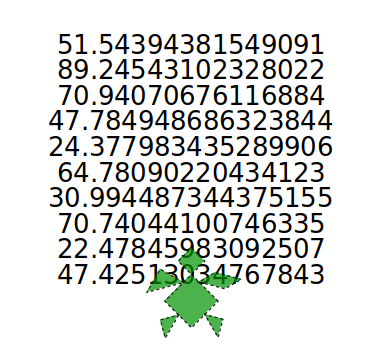
\includegraphics[width=3.0cm,trim=4 4 8 4,clip]{./images/caos-della-vita/caos-della-vita-1.png}
\label{dec-2}
\end{figure}
\end{minipage} \hfill

\vskip 1cm

With this code the Turtle first goes next to the page top, then writes a column of ten successive random numbers between 0 and 100, printing them by means of the LABEL instruction. Of course you can change whatever you like in this piece of code - it's always good to experiment.

Now, let's take a basic piece of code we are using several times, with variants:

\vskip 1cm

\begin{scriptsize}
\begin{minipage}{0.50\textwidth}
\begin{itemize}[itemsep=-3pt,parsep=2pt, leftmargin=-0.0mm ]
\item[] TO QUADRATO
\item[] \hspace{8pt} REPEAT 4 [
\item[] \hspace{8pt}\hspace{8pt} FORWARD 100
\item[] \hspace{8pt}\hspace{8pt} RIGHT 90
\item[] \hspace{8pt} ]
\item[] END
\item[]
\item[] QUADRATO
\end{itemize}
\end{minipage}
\end{scriptsize}

\vskip 1cm

This is the code to draw a square, as we have seen at the beginning of chapter \ref{cap:disegnare}. In chapter \ref{cap:ripetere} we investigated how to transform this code to get any kind of regular polygons. In a somewhat more complex variant, in chapter \ref{cap:marta}) we will explore more general cycles properties and in chapter \ref{cap:cerchio} we will discover the natural way of drawing a circle in the Turtle Geometry perspective, put in a practical didactic perspective: here just the code, to point out the similarity with the previous one.

\vskip 1cm

\begin{scriptsize}
\begin{minipage}{0.50\textwidth}
\begin{itemize}[itemsep=-3pt,parsep=2pt, leftmargin=-0.0mm ]
\item[] TO CERCHIO
\item[] \hspace{8pt} REPEAT 360 [
\item[] \hspace{8pt}\hspace{8pt} FORWARD 1
\item[] \hspace{8pt}\hspace{8pt} RIGHT 1
\item[] \hspace{8pt} ]
\item[] END
\item[]
\item[] CERCHIO
\end{itemize}
\end{minipage}
\end{scriptsize}

\vskip 1cm

Now, we have all the ingredients to give life to our Turtle. Let's inject a dose of randomness in the previous code. Within the repeating cycle, first we are going to tell the Turtle to move forward by a random amount between 1 and 2. In order to achieve this effect we write the instruction FORWARD RANDOM(1) + 1. Here we are telling the Turtle to move forward by a quantity equal to RANDOM(1) +1. The command RANDOM(1)\footnote{At the beginning we showed a slightly different syntax: RANDOM 1 instead RANDOM(1). The first one is the standard LibreLogo version reported in the official LibreLogo Toolbar manual. The second one is an alternative version which is based on the underlying python code by means of which LibreLogo has been written. In the example we are discussing this version is preferable because it gives more clarity. Actually, with the expression RANDOM 1 + 1 it is not clear if we are willing to sum 1 to the result of RANDOM 1 or if we want to call RANDOM 2. By using RANDOM(1) + 1 there is not such an ambiguity. } renders a random number between 0 and 1, thus, if we sum 1 to this, we obtain a random number which is comprised between 1 and 2. Second, we tell the Turtle to turn by a random amount, say between -45 and 45 degrees. We can achieve this result simlarly, by means of the instruction LEFT RANDOM(90) - 45, since with RANDOM(90) - 45 we get a random number between -45 and 45 degrees.

Here we have the whole piece of code and its result:

\vskip 1cm

\begin{scriptsize}
\begin{minipage}{0.50\textwidth}
\begin{itemize}[itemsep=-3pt,parsep=2pt, leftmargin=-0.0mm ]
\item[] TO RANDOMMOVE
\item[] \hspace{8pt} REPEAT [
\item[] \hspace{8pt}\hspace{8pt} FORWARD RANDOM(1) + 1
\item[] \hspace{8pt}\hspace{8pt} RIGHT RANDOM(90) - 45
\item[] \hspace{8pt} ]
\item[] END
\item[]
\item[] RANDOMMOVE
\end{itemize}
\end{minipage}
\end{scriptsize}
\begin{minipage}{0.5\textwidth}
\begin{figure}[H]
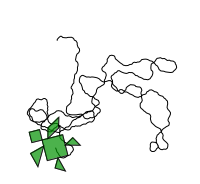
\includegraphics[width=3.0cm,trim=4 4 8 4,clip]{./images/caos-della-vita/caos-della-vita-2.png}
\label{dec-2}
\end{figure}
\end{minipage} \hfill

\vskip 1cm

If these code modifications sound weird to you, just play with it. That is copy the code in a new LibreOffice document, try to run it, then try to modify the various numbers and reflect upon what's happening.

But be aware: if you are going to run repeatedly the same piece of code you will not be able to reproduce this drawing, or better: the probability of reproducing the same drawing is extremely low. So what? How can we be happy of producing unpredictable results by means of a machine conceived for making complex and accurate calculations? Well, actually, we are very glad because with this simple code we open a windows on the huge and crucial world of scientific simulation. Nowadays, in every scientific field the simulation is an essential investigation tool, the unique possible to face the overwhelming complexity of natural phenomena. However, nowadays does not mean right today. My graduation thesis in physics, in the seventies, was heavily based on the use of computer simulation of radiation scattering within the human body. A too complex context to be faced with the tools of mathematical analysis. In physics computer simulations make use of so called Monte Carlo Methods, a broad class of computational algorithms that rely on repeated random sampling to obtain numerical results. For instance, in my thesis work, I simulated a source of radioactivity within the body, by reproducing the emission of photons, thus invoking a random number generator for any random step, such as direction of emission, interaction with matter, direction of deflection and so on.

But simulations are not restricted to the domain of physics, on the contrary, the more complex the phenomena the more simulations may turn out to be the unique possible investigation tool. In the context of biological disciplines we talk about \textit{in silico} experiments, referring to the fact that they are realized through calculations done with digital computers that run on silicon chips - the expression is an allusion to the latin phrases \textit{in vivo}, \textit{in vitro} and \textit{in situ}, commonly used in biology. Nowadays \textit{in silico} experiments include molecular biology, genetic assays, tumour growth, dermatology, bone remodelling, organ failure, clinical trials, just to mention some. In medicine, for instance, \textit{in silico} studies are used to discover new drugs because it is faster and costs much less. In biology they are used to study to formulate behaviour model of cells and in genetics to analyze gene expression\footnote{In molecular biology "gene expression" means the way a set of genes determines the functioning of the cell at the macromolecular level}.

But what are we simulating with our piece of code? The obvious answer is a turtle wandering randomly. Of course, if we imagine to observe an animal from the height in its environment, the impression will be that of a random movement. In this sense our code could be considered a simulation of the animal behaviour, even if a very poor one, since our randomness assumption is based on the fact that we ignore what the animal is actually doing. Animals move because they are looking for food or a mate, for instance. Or, perhaps, the simulation could be more appropriate for a drunk hanging around in the night, looking for a nonexistent happiness. The distribution of food for a given specie of animals in its natural environment could be modeled, in some extent, but the inner struggle of a man is much more difficult to translate in mathematical terms.

But what does it mean exactly by "modeling something", such as food distribution, in the context of our example? Yes, apparently, we injected a drop of life in our code, reproducing a randomness which we all experience in our life, in the shape of good or bad luck. However, despite such strong perception of uncertainty, we all know that our capability of observing the outside world and of tacking decisions, is crucial, as well. In substance, our turtle is totally passive! It just have some energy to proceed and to turn: no smell, no sight, no decisions. This is the point: we need a way to let the Turtle have the ability to take decisions!

Before going on learning how to let the Turtle take decisions, we diverge a bit from the LibreLogo environment to have a fast look to the fascinating world of \textit{multiple turtles}. We have to give up to LibreLogo for a while because it does not allow to run more turtles simultaneously, at least in the current version. It is plenty of Logo versions out there, and some of them allow to run more then one turtle at a time. As we have already said, the reason for using LibreLogo as the first, even if not trivial, introduction to Logo relies in its extremely \textit{low floor}, which is crucial for using it in primary school.

\vskip 1cm

\begin{scriptsize}
\begin{minipage}{0.70\textwidth}
\begin{itemize}[itemsep=-3pt,parsep=2pt, leftmargin=-0.0mm ]
\item[] clear()
\item[] invisible()
\item[] 
\item[] def path(t: Turtle, delay: Int) = runInBackground \{
\item[] \hspace{8pt} t.setAnimationDelay(delay) \{
\item[] \hspace{8pt} repeat(10000) \{
\item[] \hspace{8pt}\hspace{8pt} t.forward(random(1) + 1)
\item[] \hspace{8pt}\hspace{8pt} t.right(random(90) - 45)
\item[] \hspace{8pt} \}
\item[] \}
\item[] val t1 = newTurtle(0, 0)
\item[] t1.setPenColor(red)
\item[] val t2 = newTurtle(0, 0)
\item[] t2.setPenColor(orange)
\item[] val t3 = newTurtle(0, 0)
\item[] t3.setPenColor(yellow)
\item[] val t4 = newTurtle(0, 0)
\item[] t4.setPenColor(green)
\item[] val t5 = newTurtle(0, 0)
\item[] t5.setPenColor(blue)
\item[]
\item[] path(t1, 50)
\item[] path(t2, 50)
\item[] path(t3, 50)
\item[] path(t4, 50)
\item[] path(t5, 50)
\end{itemize}
\end{minipage}
\end{scriptsize}
\begin{minipage}{0.3\textwidth}
\begin{figure}[H]
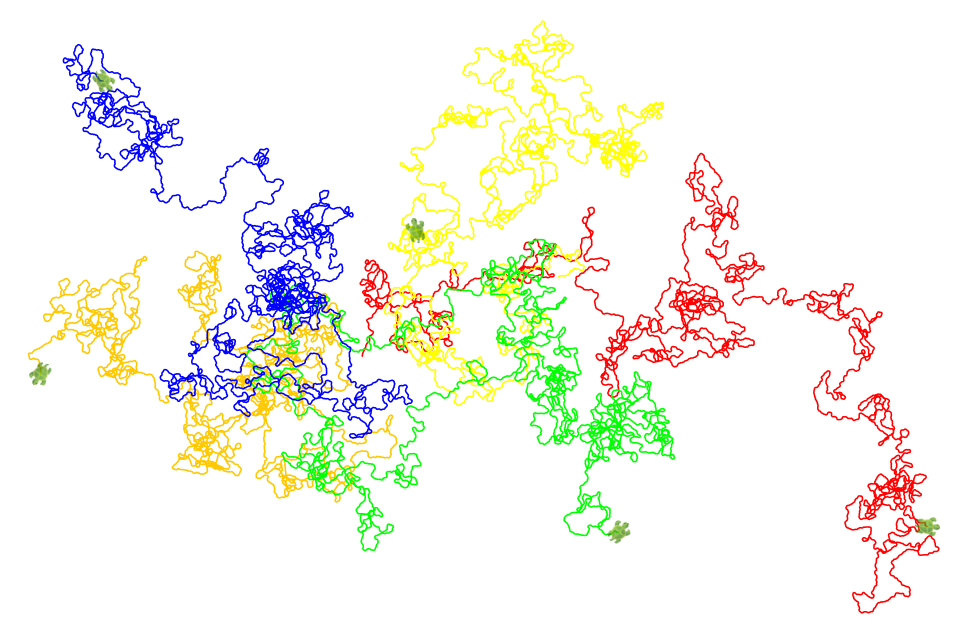
\includegraphics[width=3.0cm,trim=4 4 8 4,clip]{./images/caos-della-vita/caos-della-vita-3.png}
\label{dec-2}
\end{figure}
\end{minipage} \hfill

\vskip 1cm

In this piece of Kojo Logo code there are instructions that do not belong to the standard set of Logo commands, and precisely those that allow for controlling different turtle simultaneously. However, the standard Logo commands are pretty similar between the two systems. In the appendix in chapter \ref{cap:appendice-2} there is a little vocabulary. 



